\chapter{Discussion}

This chapter shows the results obtained during the evaluation and the tests we made to ensure the effectiveness of our models. 

\section{Testing flow?}

We write a function to execute different tests using different classificators and hyperparameters. 

As mentioned in Section \ref{sec:cv}, we used the \texttt{StratifiedKFold} class from \textit{Scikit-learn} to cross-validate our tests. This class has a method \texttt{split} that, given the train and test subsets, it returns a range of indexes to select only a portion of the dataset, as shown in Figure \ref{fig:stratified}.  At each fold, different parts of the dataset are chosen as a test subset, but summing the test subset in all the folds, we would obtain the entire dataset. Therefor we create two arrays where, at each fold, we append the predictions made by the classification model and the ones expected. At the end of the cross-validation algorithm, we use the \textit{Scikit-learn} functions \texttt{classification\_report}, \texttt{confusion\_matrix}, and \texttt{accuracy\_score}, with the complete arrays of predictions and expected values, to obtain the metrics needed to evaluate the model.

We chose $k = 10$ because, as shown in literature [cita quaclouno], it's the best value between performances and execution time. 
We set the \texttt{StratifiedKFold} option \texttt{shuffle} to true, so every time the cross-validation algorithm samples different binaries at each fold, avoiding that classification model focuses only on a very good or lousy subset of the dataset. Furthermore, we repeat each test 5 times, and then we average the results obtained.

For \texttt{RandomForest} and \texttt{XGBoost} models, we found that 300 trees are sufficient to get great results.

\section{Features selection}
In Section \ref{sec:feat_sel}, we presented different methods for feature selection. In this section, we analyze and compare them to find the best subset of features to represent APT malware.

\subsection{Scaling dataset}
The first step for selecting features is to scale the dataset. It is essential because, in our case, we have features with very different scales and contain some outliers. These two aspects can decrease the predictive performance of the classification model. We chose the \texttt{MaxAbsScaler} from \textit{scikit-learn} because it fits our needs. The scaler does not shift or center the data, and it does not destroy the sparsity of the features. For each feature, the algorithm calculates the maximum value and scales all the features in the column, such that the maximum value is equal to 1.0. All the features will be in the range of 0 and 1.0, but they maintain their variance.

\subsection{Remove low variance}
The second step is to visualize the variance of the dataset. We calculated with the std function on axis 0, and we visualize them with matplotlib. Figure \ref{fig:var_all} shows the variance of the entire dataset. As we can see, some features have zero variance, and this means that they are constant over all the samples. Thus they are not useful for classification.

\begin{figure}[!h]
	\centering
	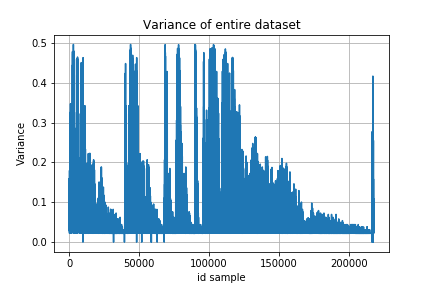
\includegraphics[width=0.6\columnwidth]{variance-all.png}
	\caption{Variance of features in the entire dataset}
	\label{fig:var_all}
\end{figure}

To remove them we use \texttt{VarianceThreshold} class that removes all low-variance features. Is it possible to set a threshold, if a feature variance is below the threshold, then it is removed. By default, the class removes all zero-variance features. This method removes \textbf{32} features from our dataset.

\subsection{Filter methods}

Filter methods works by selecting the best features based on a ranking function. Scikit-learn offers various scoring functions, such as \textit{chi2, f\_classif, mutual\_info\_classif}. To choose the best $k$ features scikit-learn has two classes:
\begin{itemize}
	\item \texttt{SelectKBest: }removes all but the highest $k$ scoring features.
	\item \texttt{SelectPercentile} removes all but a user-specified highest scoring percentage of features.
\end{itemize} 
We use \texttt{SelectPercentile} to select the best $25\%$ features with each scoring function, and we compare them in the Figures \ref{fig:chi2-flcassif}.


The chi-square function was the fastest, it only takes 7.46s to select the best features, against 246.50s of fclassif. But fclassif function performs slightly better. All the results are summarized in Table \ref{tab:rank_function}

\begin{figure}[!h]
	\centering
	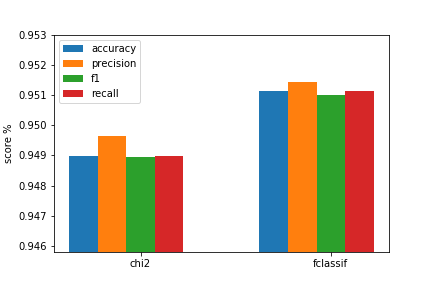
\includegraphics[width=0.6\columnwidth]{chi2-fclassif.png}
	\caption{Comparison of metrics between fclassif and chi2 ranking function}
	\label{fig:chi2-flcassif}
\end{figure}

\begin{table}[!htb]
	\centering
	\caption{Summary of ranking functions selecting the best 25\% best features}
	\label{tab:rank_function}
	\begin{tabular}{lll}
		\toprule
		\textbf{Metrics}  & \textbf{chi2} & \textbf{fclassif }\\
		\midrule
		\texttt{Time elapsed} & 7.60s & 246.05s\\
	
		\texttt{Accuracy} & 94.90\% &  95.11\%      \\ 
		\texttt{Precision}  & 94.96\% & 95.14\%          \\ 
		\texttt{F1-score}  &   94.89\%   & 95.10\%          \\ 
		\texttt{Recall} & 94.90\%  &   95.11\%       \\ 
					\bottomrule
	\end{tabular}
	
\end{table}



